\documentclass[10pt,letterpaper]{article}
\usepackage[margin=0.85in]{geometry}
\usepackage{graphicx,booktabs,amsmath,hyperref}
\hypersetup{colorlinks=true,urlcolor=blue,linkcolor=blue}
\setlength{\parindent}{0pt}
\setlength{\parskip}{6pt}
\setlength{\emergencystretch}{1em}
\setlength{\tabcolsep}{5pt}
\newcommand{\code}[1]{\texttt{#1}}
\title{\vspace{-1.7cm}CSE498 Project 3:\\Language-Guided TurtleBot3 Navigation\\with LocateAnything}
\author{Ling Shen}
\date{October 4, 2026}
\begin{document}
\maketitle
\vspace{-0.7cm}
\begin{center}\small
Project repository: \url{https://github.com/lllingshen/project3a}\\
Demo video directory: \href{https://github.com/lllingshen/project3a/tree/main/demo_video}{\code{demo\_video/}}
\end{center}
\section{System overview}
This project adds LocateAnything to the course's TurtleBot3 navigation system so that a command can select an object by its appearance. Gazebo simulates the room, robot, camera, and laser scanner. ROS 2 nodes use the sensor data to build a map, locate objects, and navigate with Nav2.

A user publishes a string to \code{/user\_command}, for example \emph{Move to the red chair.} The coordinator pauses exploration, cancels conflicting navigation, waits for Nav2 to become idle, and forwards the command. A launch parameter selects exactly one target-selection mode. Both modes reuse the same target message, approach-pose adapter, coordinator, and Nav2 backend.

\begin{center}\small
\fbox{\begin{minipage}{0.93\linewidth}\centering
User command $\rightarrow$ coordinator: pause and select mode\\[4pt]
\begin{tabular}{p{0.43\linewidth}|p{0.43\linewidth}}
\textbf{Baseline} & \textbf{LocateAnything}\\
Category/index parser + semantic landmarks & Full description + stationary RGB snapshot\\
YOLO detections feed object memory & Model box + matched LiDAR + saved TF\\
\end{tabular}\\[5pt]
Selected instance in \code{map} $\rightarrow$ approach pose $\rightarrow$ Nav2\\
SLAM occupancy map + robot pose support planning and motion
\end{minipage}}
\end{center}

In baseline mode, the parser recognizes configured categories, aliases such as ``trash can,'' and an optional index such as \code{person\_2}. Without an index, it selects the nearest matching landmark relative to the robot's current map position. An index selects that exact observed memory ID. IDs reflect observation order, not personal identity. The parser does not model color: both red-chair and blue-chair descriptions reduce to category \code{chair}. The live comparison is discussed in Section~\ref{sec:contributions}.

The detector loads the course's \code{tb3det\_yolo26n.pt} once; \code{infer()} returns label, confidence, and pixel bounding box in the wrapper's existing format. Its classes are \code{person}, \code{trash\_can}, and \code{chair}, with a detection threshold of 0.40. The detector publishes boxes and a debug image through the existing ROS wrapper. A direct test of the original stub on a blank $480\times640$ image returned no detections and \code{is\_loaded=False}.

The project is based on \href{https://github.com/YiyuchenHu/turtlebot3-gazebo-navigation-hw}{Yiyuchen Hu's course repository} (\code{a048d1e50e18}). I reused detector methods, box parsing, and geometry helpers from \href{https://github.com/lllingshen/turtlebot3-semantic-research}{my earlier research repository} (\code{694fff69d878}). The model runs through \href{https://github.com/NVlabs/Eagle}{NVIDIA Eagle} (\code{8442db3b79f7}) with local \href{https://huggingface.co/nvidia/LocateAnything-3B}{LocateAnything-3B} weights. The course history and licenses are retained. The chair mesh is by Wan Yi Seow/Open Robotics under CC BY 4.0; the red and blue material changes are listed in NOTICE. Full source commits and run records are in \code{report/results.json}.

\newpage
\section{Visual grounding and navigation} SLAM Toolbox uses laser scans and robot motion to estimate pose and construct an occupancy grid: cells indicate free, occupied, or unknown space. Semantic memory adds labeled object landmarks such as \code{person\_2}. It associates repeated detections and retains map positions. The occupancy grid supports path planning, while semantic memory connects object labels to locations in that grid.

In LocateAnything mode, the baseline query node is not launched. A persistent worker in a separate Python environment loads the existing local LocateAnything-3B model. The complete referring expression is preserved: only the leading movement phrase is removed. For the red command the actual prompt was:
\begin{quote}\small
Locate a single instance that matches the following description: the red chair.
\end{quote}
The selected box is localized and sent directly to navigation. YOLO can continue updating semantic memory during this process without changing the selected target. Each selection has its own \code{locateanything\_N} ID.

Before inference, the robot stops and the node captures a camera image, CameraInfo, a nearby laser scan, odometry, and timestamped transforms. The sensor matching tolerance is 0.15~s; stale images and motion during inference are rejected. The image keeps its original timestamp, and the transforms are saved before inference so that localization uses the pose at capture time.

Model coordinates use a 0--1000 scale. They are converted to the original $W\times H$ camera pixels by $u=xW/1000$, $v=yH/1000$. For box center $(u_c,v_c)$ and camera intrinsics, the optical ray is
\[
\mathbf r_c=\big((u_c-c_x)/f_x,\;(v_c-c_y)/f_y,\;1\big).
\]
The camera-to-scan rotation gives a planar bearing $\theta$. Nearby valid laser returns inside the box's angular width provide a median range $d$. The scan-frame point $(d\cos\theta,d\sin\theta,0)$ is transformed into \code{map} using the saved scan-time TF. This reuses the research localizer's planar approximation; it assumes the requested object intersects the laser plane and ignores the small camera-to-laser translation when forming the ray.

The selected metric point is sent directly in \code{SemanticQueryResult}. The adapter computes a 0.5~m standoff along the current robot-to-target direction in the same frame. Nav2 uses the occupancy map, costmaps, and localization to plan and execute the approach. The coordinator tracks success/failure and automatically re-enables exploration after a delay. In the mapped chair demonstration, exploration nodes are intentionally disabled; the observed ``exploration resumed'' status is a coordinator state transition, not an exploration-motion test.

If the model returns an invalid or ambiguous box, or the sensor data and transforms cannot support localization, the command fails without sending a goal. The required message field \code{confidence=1.0} is a placeholder and should not be read as a model confidence score.

\newpage
\section{Red and blue chair demonstrations}
A compact room contains two copies of the same course VisitorChair mesh with different red and blue materials. Both are visible from the starting pose and have the original solid collision geometry. For either command, the other chair serves as a distractor. The robot is reset between commands, and the map is available before grounding.

\begin{figure}[ht]
\centering
\begin{minipage}{0.485\linewidth}\centering
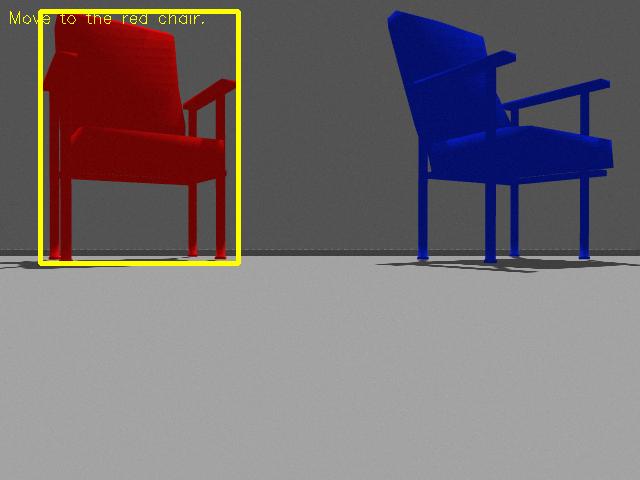
\includegraphics[width=\linewidth]{figures/red-chair.png}\\[-1pt]
\small (a) Move to the red chair.
\end{minipage}\hfill
\begin{minipage}{0.485\linewidth}\centering
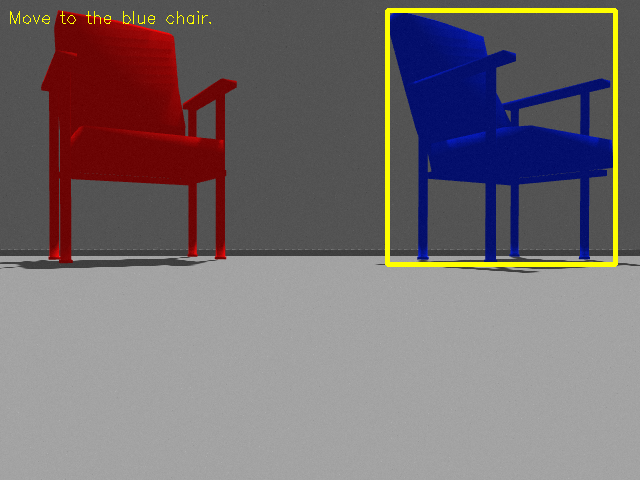
\includegraphics[width=\linewidth]{figures/blue-chair.png}\\[-1pt]
\small (b) Move to the blue chair.
\end{minipage}
\caption{Camera images from the two runs. LocateAnything selects the chair named in the command while the other chair remains visible.}
\end{figure}

\begin{table}[ht]\centering\small
\begin{tabular}{lrrrr}
\toprule
Requested target & Inference & To terminal & Final distance & Arrival\\
 & (s) & (s) & (m) & $\leq1.2$~m\\
\midrule
Red chair & 0.168 & 8.079 & 1.080 & Pass\\
Blue chair & 0.184 & 7.405 & 1.170 & Pass\\
\bottomrule
\end{tabular}
\caption{Final red and blue runs, with baseline detection and memory still running. Time to terminal includes grounding and navigation; inference time excludes the 4.697~s model load.}
\end{table}

Both commands produced a box around the requested chair and led to that same chair during navigation. The selected map coordinates were $(0.858,0.727)$ for red and $(0.776,-0.691)$ for blue. Source image-to-scan offsets were 94~ms and 10~ms. Selected-point discrepancies from the Gazebo chair origins were 0.339~m and 0.434~m. These include the difference between the observed near surface and the model origin; they are not direct estimates of sensor accuracy.

Arrival was checked using the robot and object world poses from Gazebo, sampled after navigation ended and before exploration resumed. The planar distance must be at most 1.2~m, as required by the course. The distance to the other chair was 1.623~m for the red run and 1.648~m for the blue run. Gazebo object poses are used only by this evaluator, never by grounding, target selection, or goal generation.

Four earlier attempts also passed, and all six runs are included in \code{results.json}. These runs demonstrate selection between the two colored chairs, but are too limited to establish a general success rate. The final blue run finished only 0.030~m inside the distance limit.

\newpage
\section{Results and discussion}
\label{sec:contributions}
All nine packages built successfully. The detector and integration checks passed, including 40 tests and a separate ROS navigation-cancellation test. The live detector self-test passed. Generic \code{go to person} reached the center person at 0.702~m. Commands for observed IDs \code{person\_0} and \code{person\_1} reached northwest and southeast people at 0.672~m and 0.688~m. The corrected trash-can run passed at 0.726~m. Exploration resumed after each successful baseline run.

The baseline chair test needed assistance. Unaided exploration for 600~s left the chair mislabeled as a trash can, and \code{go to chair} failed with no chair landmark. After an ordinary memory-based reposition command, an operator turned the camera toward the chair and held still for 22~s. The unchanged detector/memory then relabeled it; a new chair command reached the correct chair at 0.973~m and exploration resumed. The chair result therefore demonstrates navigation after assisted observation, not fully autonomous discovery. This used the normal memory update process, with no injected landmarks, ground-truth goals, or threshold changes.

\begin{figure}[ht]\centering
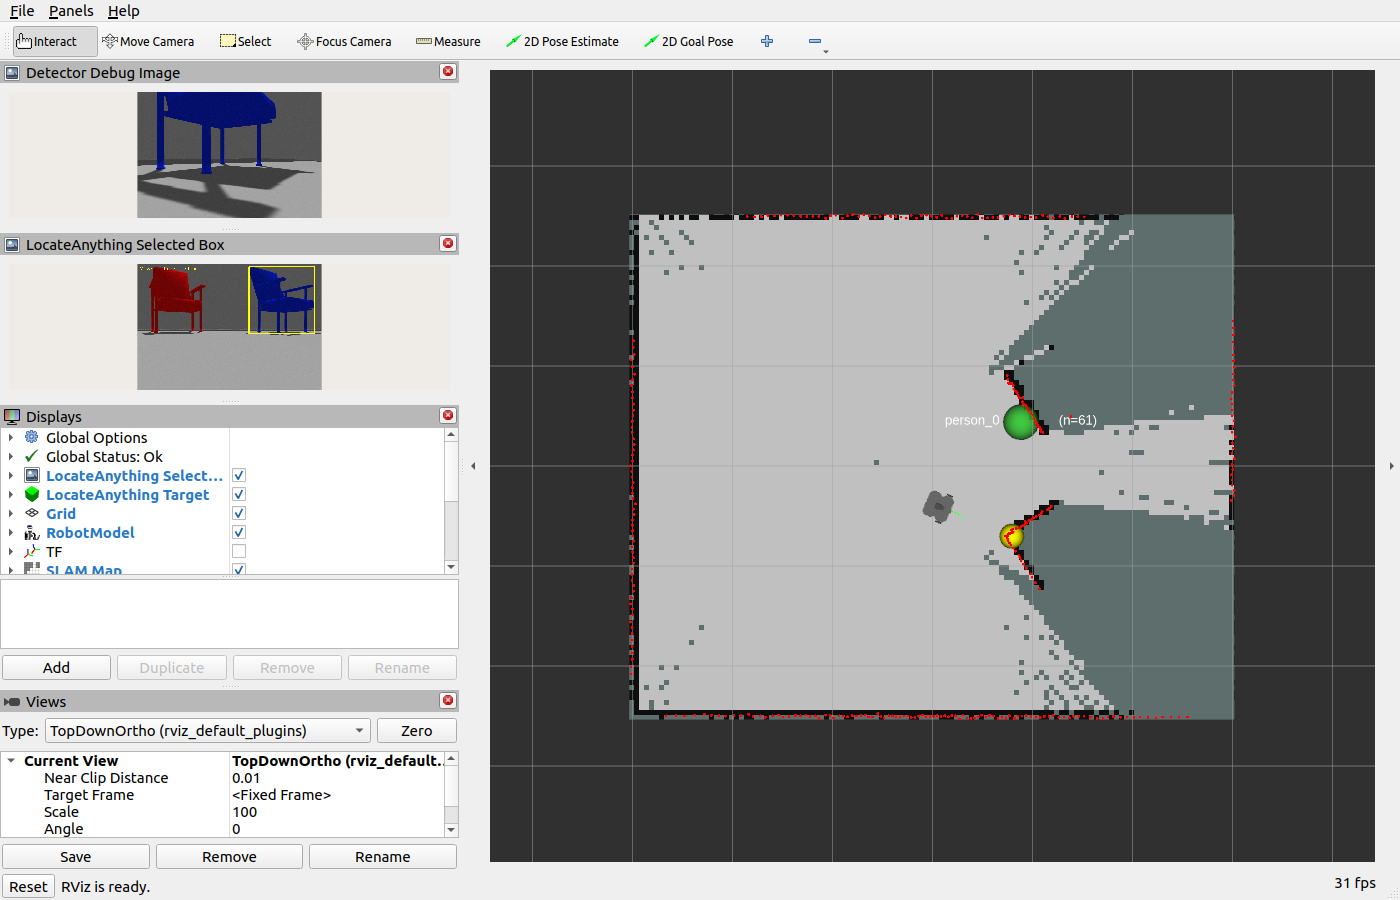
\includegraphics[width=0.66\linewidth,trim=0 240 0 50,clip]{figures/rviz-blue-arrival.png}
\caption{RViz after the second blue-chair run (cropped). The saved box and yellow marker show the selected chair. The green \code{person\_0} marker is the baseline's incorrect label for the red chair.}
\label{fig:rviz}
\end{figure}

In the same colored-chair scene, both baseline commands failed with ``no active chair in memory''. The detector labeled the red chair as a person. Although the baseline parser also ignores color, this comparison reflects detection and memory errors as well as the difference in language handling. The blue run additionally encountered an unavailable map transform in the evaluator.

Some earlier checks also failed. The first generic-person run had missing Gazebo pose queries; a later query of the stationary objects gave a supplemental distance of 0.751~m, with the original failure kept in the record. The first trash-can command selected a mislabeled chair and stopped 2.096~m from the intended trash can. A retry selected the right region but aborted (2.090~m). Waiting for cancellation acknowledgement and Nav2 idle fixed that handoff race; the later trash-can run passed. The failed attempts and subsequent checks are included in \code{results.json}.

My main contribution is connecting the full description and camera image to the target used by the existing navigation system. I completed the detector, added the persistent LocateAnything worker and synchronized localization, and created the colored-chair scene. I also corrected the robot-relative target selection and approach pose, and the cancellation and message-ordering issues encountered during testing. The project continues to use the course's ROS interfaces and Nav2 planner.

Tests ran on Ubuntu 22.04 with ROS 2 Humble, an RTX 5090, PyTorch 2.7.1+cu128, Ultralytics 8.4.60, and NumPy 1.26.4. The current extension requires a mapped scene and a visible, stationary target that intersects the laser plane. Searching for unseen objects and reliable rejection of absent targets remain outside this project.

The \href{https://github.com/lllingshen/project3a}{project repository} contains the code, report, and README launch instructions. Its \href{https://github.com/lllingshen/project3a/tree/main/demo_video}{\code{demo\_video/}} directory is the location for the recorded demonstration of \emph{Move to the red chair.} and \emph{Move to the blue chair.}
\end{document}
